\chapter{Background}
\section{The World Wide Web}
The World Wide Web is the greatest repository of information ever assembled by
man. It contains knowledge in the form of documents and multimedia resources concerning almost every area or subject regarding our lives. All this data is freely accessible to anyone with an Internet connection. It’s success is largely due to its decentralized design and nature. Web pages are hosted by different computers and each document can point to other documents independent of where the other document is physically located. As a result everybody all over the world can publish content on the web, allowing it to grow exponentially as more and more people learn how to use it.

However the huge scale of the web leads to some consequences. Due to the sheer volume of available information, it is becoming increasingly difficult to locate useful
information. Although search engines, e.g Google, Yahoo, Bing,  can provide some assistance, they are far from perfect. For many users, locating the "right" document is still like trying to find a needle in a haystack.

\subsection{Development of the Web}
In 1990 Tim Berners-Lee developed the first version of his World Wide Web
program at CERN. The concept behind his invention was to use hypertext as a means of organizing a distributed document system. The term \textit{hypertext} refers to a collection of documents with references to each other (links) that enable readers to navigate from one document to the other without following a sequential pattern. In order to make it work on the Internet, Berners-Lee had to develop three crucial parts of the whole system:
\begin{enumerate}
    \item Mechanism for addressing documents on different machines.
    \item Protocol that allowed computers to request documents.
    \item Simple language to describe the documents.
\end{enumerate}
 Before inventing the World Wide Web there were more powerful hypertext systems available, but he built his according to simple specifications that he later published as standards. That enabled other people to use his system in their own web servers, web browsers and especially integrate them in their own websites. In time his system proved to be the most popular and most used in the world and that is why he founded W3C (World Wide Web Consortium) in order to oversee these standards and evolve them in the future.

\subsection{Enabling Technologies}
\subsubsection{HTTP}
Hypertext Transfer Protocol (HTTP) is a method for encoding and transporting information between a client (e.g. a web browser) and a web server. HTTP is the primary protocol for transmission of information across the Internet. Information is exchanged between clients and servers in the form of hypertext documents, from which HTTP gets its name. Hypertext is structured text that uses logical links (hyperlinks), between nodes containing text. Hypertext documents can be manipulated using the Hypertext Markup Language (HTML). Using HTTP and HTML clients can request different kinds of content (such as text, images, video, and application data) from web and application servers that host the content.

HTTP follows a request-response paradigm in which the client makes a request and the server issues a response that includes not only the requested content, but also relevant status information about the request in the form of \textit{headers}. This self-contained design allows for the distributed nature of the Internet, where a request or response might pass through many intermediate routers and proxy servers. It also allows intermediary servers to perform value-added functions such as load balancing, caching, encryption, and compression. HTTP resources such as web servers are identified across the Internet using unique identifiers known as Uniform Resource Locators (URLs). HTTP is an application layer protocol and relies on an underlying network-level protocol such as Transmission Control Protocol (TCP) to function.

\subsubsection{HTML}
HTML is a markup language designed for the web as a way to structure documents semantically. Web browsers can read HTML files and render them into visible or audible web pages. Internally HTML describes a hierarchical structure depicted from the ability to nest tags within each other. This structure is called the Document Object Model (DOM) and plays an important role when manipulating HTML with Javascript for achieving web page interactivity. HTML5 is the newest standard which adds many new features to the language such as native support for including and handling multimedia and graphical content - the new \verb|<video>|, \verb|<audio>| and \verb|<canvas>| elements, support for Scalable Vector Graphics (SVG) content and MathML for mathematical formulas. Another neat feature are semantic tags used to enrich the semantic content of documents, new page structure elements such as \verb|<main>, <section>, <article>, <header>, <footer>, <aside>, <nav>| and \verb|<figure>| are added.  

\subsubsection{CSS}
Cascading Style Sheets (CSS) is a style sheet language used for describing the presentation of a document written in a markup language. CSS is designed primarily to enable the separation of document content from document presentation, including aspects such as the layout, colors, and fonts. This separation can improve content accessibility, provide more flexibility and control in the specification of presentation characteristics, enable multiple HTML pages to share formatting by specifying the relevant CSS in a separate .css file, and reduce complexity and repetition in the structural content.

\subsubsection{Javascript}

Javascript is a dynamic programming language originally designed for the web and standardized in the \textit{ECMAScript} language specification. It is a multi-paradigm language, supporting imperative, object-oriented and functional programming. Functions are treated as first class citizens. A lot of language constructs are inspired by languages such as Java and Scheme. Although meant to live in the browser, Javascript has proven over time to be suitable as a general-purpose programming language. NodeJS is an example of a runtime environment allowing to use Javascript for server side development, MongoDB accepts queries written in Javascript, Adobe's Acrobat and Adobe Reader support JavaScript in PDF files etc..

\section{Knowledge Representation}
Knowledge Representation is a field of artificial intelligence that deals with the symbolic representation of knowledge of a subject area. This is accomplished in an automatic way by using reasoning programs. More informally, it is a part of AI, which is concerned with thinking and how thinking leads to intelligent behavior. As a field of study, it proposes an approach to understanding Intelligent behavior that is radically different from the others. Instead of studying people or animals (their biology, their nervous system, their psychology, their sociology, their development, etc.), it is the people's knowledge that is to be studied. It is accepted that people possess the right knowledge and this knowledge can apply in different situations in order to achieve their goals. Therefore, in the range of KR you deal with knowledge and not with the owner of knowledge.

The goal is the development of formalism by which knowledge about the world can be described in an abstract way and can be effectively used to implement intelligent applications. The nature of knowledge is a difficult (philosophical) question. KR is only limited to conceptual knowledge. Other types of knowledge are temporal knowledge, spatial knowledge, procedural knowledge, knowledge of knowledge, etc. KR makes a description of the concept of a lecture, a computer, an illness, a workpiece, etc. - a "what is a XYZ" description.

\subsection{Logic in Knowledge Representation}
The main goal of logic (there is no uniform study of logic but many) is to express knowledge about a certain phenomena or a specific part of the world by means of a formal language. The core that defines reasoning about real world things is their encoding by using a precise set of deterministic rules called \textit{inference rules}, that everyone agrees upon. Correct reasoning enables particular knowledge to be represented by a logical sequence from a set of facts. In logic correct reasoning chains are constructed by chaining applications of simple inference rules that transform the original knowledge in a derived conclusion. 

\subsubsection{First Order Logic}
First Order Logic is a formalism by which one can describe statements very expressively. Just like prepositional logic, first order logic has:

\begin{itemize}
    \item a syntax that determines which strings are its valid formulas.
    \item semantics that determines the meaning of each of these formulas.
\end{itemize}

FOL deals with objects (for example, the residents of Frankfurt and their relationships or the natural numbers and their addition and multiplication) and statements about their properties. In contrast, the propositional logic deals not with objects but only with "true" and "false" statements and their combination.
The world is modeled on terms of:

\begin{itemize}
    \item \textit{Objects} - things with individial identities.
    \item \textit{Features} - characteristics of objects that distinguish an object from other objects.
    \item \textit{Relations} - connections between sets of objects.
    \item \textit{Functions} - a subset of relations, which only take one value as input.
\end{itemize}

FOL overtakes, modifies and extends the syntax of prepositional logic:
\begin{itemize}
    \item Similarities:
    \begin{itemize}
        \item Operators $\neg, \wedge, \vee, \rightarrow, \leftrightarrow$.
    \end{itemize}
    \item Differences:
    \begin{itemize}
        \item Variables do not correspond to “true” oder “false” expressions, but to elements of the universe of a  $\sigma$-structure.
        \item Variables are not atomic formulas any more.
    \end{itemize}
    \item What is new:
    \begin{itemize}
        \item Quantifiers: $\exists$ ("does exist") and $\forall$ ("for all").
        \item There are symbols for elements from the $\sigma$ signature.
    \end{itemize}
\end{itemize}
\subsubsection{Description Logic}
Description logic is a family of knowledge representation formalisms, which allow the key terms of a field to be described in a formal, logic-based language. Such types of logic are used in various applications, but especially for the semantic annotation of data in data integration and the World Wide Web. The familiar Web Ontology Language (OWL) is substantially based on a description logic. Syntax and semantics are here always well-defined logic-based:

\begin{itemize}
    \item \textit{Syntax:}  recursive definition in which the constructors that can be used to form concept terms are stated. Some constructors are related to logical constructors in first-order logic (FOL) such as \textit{intersection} or \textit{conjunction} of concepts, \textit{union} or \textit{disjunction} of concepts, \textit{negation} or \textit{complement} of concepts, \textit{universal restriction} and \textit{existential restriction}. Other constructors have no corresponding construction in FOL including restrictions on roles for example, \textit{inverse}, \textit{transitivity} and \textit{functionality}.
    \item \textit{Semantics:} strengthens the meaning of representing knowledge in a precise, unambiguous way.
    \begin{itemize}
        \item \textit{Declarative semantics:} independent from the processing, e.g. you want to represent (describe), not to program in something like Prolog. It enables widespread application independence and is based on logical structures.
    \end{itemize}
\end{itemize}
Central elements of descriptive logic are:
\begin{itemize}
    \item \textit{Concepts} - describe classes from objects.
    \begin{itemize}
        \item person, course, university, table, student, etc.
    \end{itemize}
     Can be described by using logical expressions (formulas).
    \item \textit{Roles} - binary relations between objects.
    \begin{itemize}
        \item listen, teach, partOf, etc.
    \end{itemize}
    In most cases can be described by simple expressions. 
    \item TBoxes (assertion of concepts) - define and connect concepts.
    \begin{itemize}
        \item \textit{Definition of concept}\newline 
        student $\equiv$ person $\sqcap \exists$ listens.lecture  
        \item \textit{General background knowledge / Constraint}\newline
        student $\sqcap$ lecture hall $\sqsubseteq \bot$
    \end{itemize}
    \item \textit{ABoxes (assertions of individuals)} - describe individuals (objects) and their features.
        \begin{itemize}
            \item student(hans)\newline
            lecture $\sqcap \exists$ subject.informaticsSubject(blv)\newline
            listens(hans, blv)
        \end{itemize}
\end{itemize}

\subsection{Semantic Networks and Frame Systems}
One of the oldest knowledge representation formalisms are semantic networks. Each concept in a semantic net is represented by a node in a graph. Concepts that are
semantically related are connected by arcs, which could be optionally labeled. Implication of meaning is represented by the way a concept is connected to other concepts. Special arcs are used to represent abstraction, although their semantics are often unclear. Now it is rather common to use two arcs for this purpose. An \textit{is-a} arc indicates that one concept is a subclass of another, while an \textit{instance-of} arc indicates that a concept is an example of another concept (see \textit{Figure \ref{fig:semantic_net}}). These types of arcs have correlations in basic set theory: \textit{is-a} is like the subset relation and \textit{instance-of} is like the element of that relation.
A collection of \textit{is-a} arcs specifies a partial order on classes often referred to as a \textit{taxonomy} or \textit{categorization hierarchy}. The taxonomy can be used to adjust the abstraction level - either generalize a concept to a more abstract class or specialize a class to its more specific concepts.

\begin{figure}[h!]
    \centering
    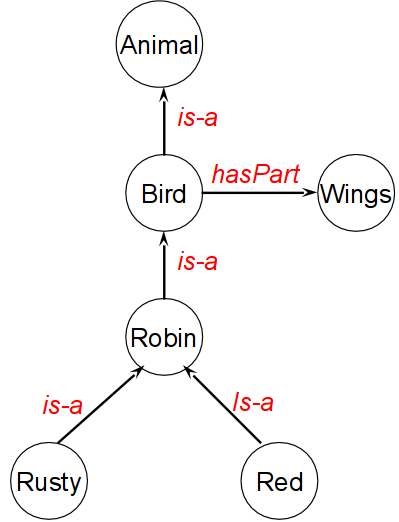
\includegraphics[width=10cm]{semantic_net}
    \caption{Semantic net inheritance}
    \label{fig:semantic_net}
\end{figure}

In the 1970's Marvin Minsky introduces frame systems. In the terminology of such systems, a frame is a named data object that has a set of slots, where each slot
represents a property or attribute of the object. Slots can have one or more values (called fillers), some of which may be pointers to other frames. Since each frame has a set of slots that represent its properties, frame systems are usually considered to be
more structured than semantic networks. However, it has been shown that frame systems are similar to semantic networks. Famous KR languages based on frame systems are KRL and KL-ONE (based on description logic). 

\subsection{Ontologies}


\section{Databases}
\subsection{Distributed Databases}
\subsection{Graph Databases}
\section{Semantic Web}
The Semantic Web reveals the next generation in the development of the Internet. It enables interconnectedness of data from one source to another and the representation of this data in a machine readable form. This way computers can understand the information and can process ever more demanding tasks. The Semantic Web consists of a stack of standards and best practices for sharing data and its semantics across the Internet in order to be used by applications. Heavily backed up by the W3C the Semantic Web is also built using the same type of standards such as, e.g. HTML and CSS. These standards are: the RDF data model, the SPARQL query language, the RDFS and OWL standards for vocabularies and ontologies. A product could be created with built-in semantics but if it does not adhere to these standards it cannot be part of the Semantic Web. 

\subsection{Resource Description Framework (RDF)}
The Resource Description Framework (RDF) is the result of the work of the W3 Consortium for a web infrastructure for metadata. It is standardized on 22.February 1999. It represents a data model with well-defined formal semantics, based on directed graphs and modelling data as a set of triples \textit{Triple (subject, predicate, object)}. A set of triples builds a graph.
\begin{figure}[h!]
    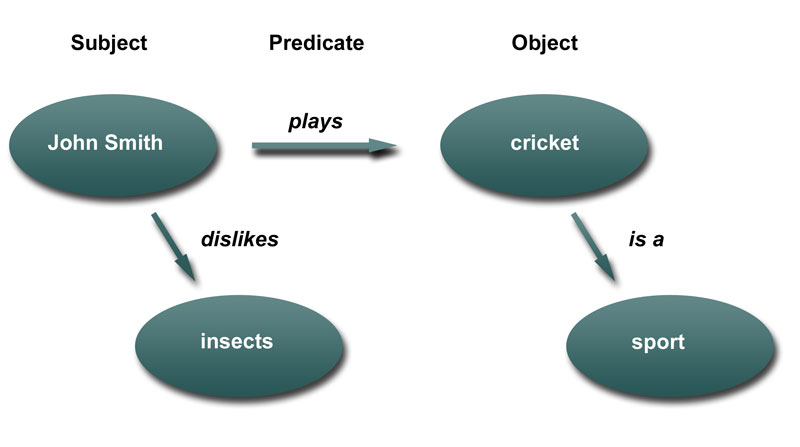
\includegraphics[width=\linewidth]{rdf-triple-example}
    \caption{RDF Triple Scheme}
    \label{fig:view}
\end{figure*}

A \textit{resource} is something that is uniquely identified and can express something about it. \textit{Subjects} und \textit{predicates} are always resources and an \textit{object} could either be a resource or a \textit{literal}. Literals could be strings or other datatypes (numbers, dates, etc.).

A crucial difference in comparison to other data models such as the relational data model is that RDF represents information as a graph and all objects are connected by edges. For example the sentence "Dresden is a city in Sachsen." partitions itself as "Dresden" and "Sachsen" being objects that are connected with the edge "is a city in". In RDF the following triple is constructed: \textit{subject (Dresden)}, \textit{predicate (is a city in)} and the \textit{object (Sachsen)}. In its essense this is everything. So why bother having this model? HTML describes the structure of a web page in a standardized fashion. This leads to strong decoupling from the used browsers when consuming web page content. The answer is that the same has to be achieved from RDF, but for data.

Data from the Web today is being provided through various custom formats and interfaces. If you want to aggregate it to find it new applications, these interfaces must be individually connected and brought up in a new individual format. In addition today lots of data is listed directly in web pages, e.g. in HTML. In order to utilize this data, it must be extracted individually from the websites. This means for a very high expenditure and also restricts the actual availability of data and sometimes associates with poorer quality. All of this changes when RDF is used because it eliminates the transformation of data since it is provided and used in the same exact model.

In addition individual graphs could be connected with new links, something understood as the \textit{"Linked Data"} concept which is all about connecting information on a topic so that it could be structurally navigated.

RDF is a data model which could be represented in different formats like e.g. XML (RDF/XML), HTML (RDFa), JSON (JSON-LD) or Turtle (a lighter more human readable format). RDF itself is schema-less, but there do exist different schemes like OWL (Web Ontology Lanquage) and RDFS (RDF Schema). There is also SPARQL (SPARQL Query Language) which is a query language like SQL but for RDF.

\subsection{Web Ontology Language(OWL)}
The OWL (Web Ontology Language) is designed to enable processing of the information content of applications instead of only presenting it to the user. OWL facilitates additional vocabulary in conjunction with formal semantics and allows stronger interpretations of web content than XML, RDF and RDFS. It consists of three languages with increasing expressiveness : OWL Lite, OWL DL and OWL Full. It differs \textit{classes, properties and instances} and works according to the open world assumption which allows  inferring new facts related to a class, even though previously you had none for this class. OWL also consists of a set of axioms which describe the classes, their properties and the relationships between them.

\subsection{SPARQL Query Language (SPARQL)}
SPARQL is a query language, i.e. a semantic query language for databases storing and manipulating RDF. It is a standard which has been created by the RDF Data Access Working Group (DAWG) of the W3C and is recognized as one of the key technologies of the Semantic Web. Although SPARQL queries RDF, it is not only limited to data in the RDF formats. Commercial and open source utilities are available for handling relational data, XML, spreadsheets and other formats such as RDF, so that you can write SPARQL queries against each of these sources or a combination of them. The "protocol" part of the SPARQL standard sets rules for clients and SPARQL processing servers on how to exchange results between each other. Those rules are specified in a document separate from the query language specification and it usually concerns only developers of SPARQL-processors.

The query in the next example finds the names of all African capitals and the countries in which they are located.

\begin{verbatim}
PREFIX abc: <http://example.com/exampleOntology#>

SELECT ?capital ?country
WHERE {
    ?x abc:cityname ?capital ;
       abc:isCapitalOf ?y .
    ?y abc:countryname ?country ;
       abc:isInContinent abc:Africa .
}
\end{verbatim}

Variables are prefixed with a "?" (a possible alternative is also "\$"). As a result the query above returns all variable assignments for "?capital" and "?country", that match the four RDF-triple patterns. Writing out the whole URIs each and every time ruins the readability of the query so that is why prefixes are used. In this case "abc:" stands for \verb|"http://example.com/exampleOntology\#"|.

\subsection{Triplestores (semantic databases)}
When you want to save lots of triples, persisting them in a huge file as Turtle or RDF/XML is probably not the brightest idea, because at this scale you will need a system that indexes your data for fast retrieval when searching and also a system that decides which parts of your data to keep in memory for optimal performance without swapping to disk.
This is exactly the job of a DBMS (Database Management System), e.g. MySQL or Oracle, but one that is optimized for RDF data. Such types of databases are called triplestores. One of the best on the market today are \textit{GraphDB from Ontotext} und \textit{Virtuoso from OpenLink}.

\begin{figure}[h!]
    \caption{Famous triplestore logos}
    \begin{subfigure}[b]{0.5\textwidth}
        \centering
        
\includegraphics[width=7.5cm]{graphdb-logo}
        \caption{Ontotext GraphDB logo}
        \label{fig:view}
    \end{subfigure}
    \begin{subfigure}[b]{0.5\textwidth}
        \centering
        
\includegraphics[width=5cm]{virtuoso}
        \caption{OpenLink Virtuoso logo}
    \label{fig:view}
    \end{subfigure}
\end{figure}

\section{Linked Data}

The term \textit{Linked Data} refers to a set of best practices for publishing and connecting
structured data on the Web. These best practices have been adopted by an increasing number of data providers over the last years, leading to the creation of a global data space containing billions of facts - the \textit{Web of Data}. 

The Web today relies on HTML documents connected by untyped hyperlinks. Linked Data on the other hand needs documents containing data in RDF format. However rather than simply connecting these documents, Linked Data uses RDF to make typed statements that link arbitrary things in the world. The result is what we refer to as the
Web of Data - a network of connected data pieces (facts) that are strongly interconnected enabling easy machine processing and new types of applications based on this technology.

There is already a lot of structured data accessible on the Web through Web 2.0 APIs, e.g. the APIs from Google, Yahoo or Amazon. Compared to them, Linked Data has the advantage of providing a single, standardized access mechanism instead of relying on diverse interfaces and result formats. This gives the following capabilities regarding data sources:

\begin{itemize}
    \item Easy crawling by search engines.
    \item Access using generic data browsers.
    \item Adds links between data from different data sources.
\end{itemize}

\subsection{Linked Data Principles}
Berners-Lee (2006) outlined a set of "rules" for publishing data on the Web in a way that all
published data becomes part of a single global data space:
\begin{enumerate}
    \item Use URIs as names for things.
    \item Use HTTP URIs so that people can look up those names.
    \item When someone looks up a URI, provide useful information, using the standards
(RDF, SPARQL).
    \item Include links to other URIs, so that they can discover more things.
\end{enumerate}

These rules have become known as the \textit{"Linked Data principles"}, and provide a basic recipe for publishing and connecting data using the infrastructure of the Web while adhering to its architecture and standards.

\subsection{Linked Open Data (LOD) project}

The most popular example of adoption and application of the Linked Data principles is
the \textit{Linked Open Data} project, a big community effort that started in January
2007 and is supported by the W3C Semantic Web Education and Outreach Group. The ongoing aim of the project is to start building the Web of Data by identifying existing data sets that are available under open licenses, convert them to RDF, according to the Linked Data principles, and publish them on the Web.

The early stages of the project involved researchers and developers from universities and small companies. Since then the project has grown
considerably and large organisations such as the BBC, Thomson Reuters and the Library of Congress started contributing to the project. This growth is enabled by the open nature of the project, where anyone can participate simply by publishing a data set according to the Linked Data principles and interlinking it with existing data sets. The figures below depict the range and scale of the whole initiative: 

\begin{figure}[h!]
    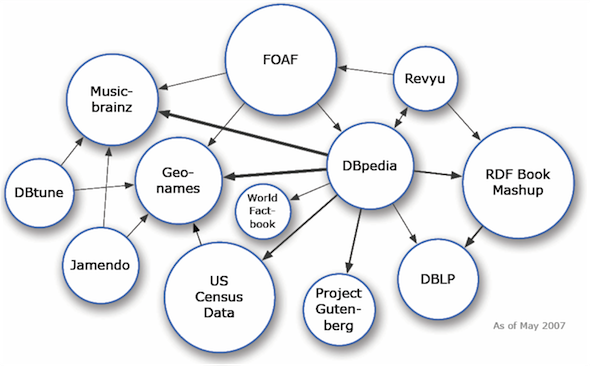
\includegraphics[width=\linewidth]{lod-cloud-may-2007}
    \caption{Linked Open Data state - May 2007}
    \label{fig:view}
\end{figure}

\begin{figure}[h!]
    \includegraphics[width=\linewidth]{lod-cloud-august-2014}
    \caption{Linked Open Data state - August 2014}
    \label{fig:view}
\end{figure}

\subsection{Publishing Linked Data on the Web}
Publishing a data set as Linked Data on the Web involves the following three basic steps:
\begin{enumerate}
    \item Assign URIs to the entities described by the data set. These entities must be retrievable (dereferenceable) from that URI over the HTTP protocol as RDF representations.
    \item Set RDF links to other data sources on the Web, so that clients can navigate the Web of
    Data as a whole by following RDF links.
    \item Provide metadata about published data, so that clients can assess the quality of published data and choose between different means of access (SPARQL endpoint, RDF dumps) besides dereferenceable URIs.
\end{enumerate}

As already stated above URIs should be valid, i.e. a request to that URI should provide the searched entity's RDF representation. Data providers can choose between two HTTP URI usage patterns to identify entities:
\begin{itemize}
    \item \textbf{303 URIs} - use a special HTTP status code, "303 See Other", to distinguish non-document resources from regular web documents. The server is configured to answer requests to such URIs with a 303 HTTP status code and a \textit{Location} header providing a new URL to a document describing the resource, e.g.:
    \begin{enumerate}
        \item Make request to \verb|http://example.com/id/alice|.
        \item Server responds with 303 status code and employs content negotiation (\verb|Accept: application/rdf+xml|, other type or none) to send either the URL of an HTML document or RDF.
        \item Requests for HTML would be redirected to \\ \verb|http://example.com/people/alice| and requests for RDF data would be redirected to \verb|http://example.com/data/alice|.
    \end{enumerate}
    \item \textbf{Hash URIs} - URIs that contain a special part called a \textit{fragment} which is usually not interpreted as part of the URI, e.g. \verb|http://example.com/data#alice|. Requesting clients will always strip off the fragment part, resulting in a request to this URI: \verb|http://example.com/data|, which will serve an RDF document describing all entities under the \verb|"data"| namespace. Again by employing content negotiation one can redirect to an HTML document \\ (\verb|http://example.com/data.html|) or other RDF descriptions \\ (\verb|http://example.com/data.rdf|).
\end{itemize}
Hash URIs have the advantage of usually making less requests in order to retrieve a whole set of RDF descriptions, but if the data set is huge and you only want to retrieve a particular description of an entity then 303 URIs are better suited due to having more fine-grained control on the server side.

In an open environment like the Web, different information providers publish data about the same real world entity like a geographic location or a person and thus introduce different URIs to identify the same entity. DBpedia uses the URI \verb|http://dbpedia.org/resource/Berlin| to identify Berlin, while Geonames uses the URI
\verb|http://sws.geonames.org/2950159/| to identify Berlin. As both URIs refer to the same thing, they are called URI aliases. URI aliases are common because it cannot be expected that all information providers agree on the same URIs to
identify an entity. URI aliases also provide an important social function to the Web of Data
as they are dereferenced to different descriptions of the same entity and allow different views and opinions to be expressed. In order to still be able to track these diverse opinions, it is a common
practice that data providers set \verb|owl:sameAs| links to all URI aliases they know about.

\subsection{Linked Data Applications}